\chapter{Programming - Check Program}
\section{Overview}\paragraph*{The Programming -}\textbf{ Check Program} screen 1 (Figure 9.1) provides the Operator a table view of the \textbf{Block Program Details} they entered to be used while in \textit{Auto} mode. The Operator is able to \textbf{\textit{Clear Program Contents}} and \textbf{\textit{Reset Auto Sequence}} from this screen. Navigation is possible to the main \textbf{Alarm} screen, the \textbf{PREV} screen (Block Program), the \textbf{NEXT} screen (next Check Program), and of course the \textbf{Main} operation screen.
\begin{figure}
	\centering
	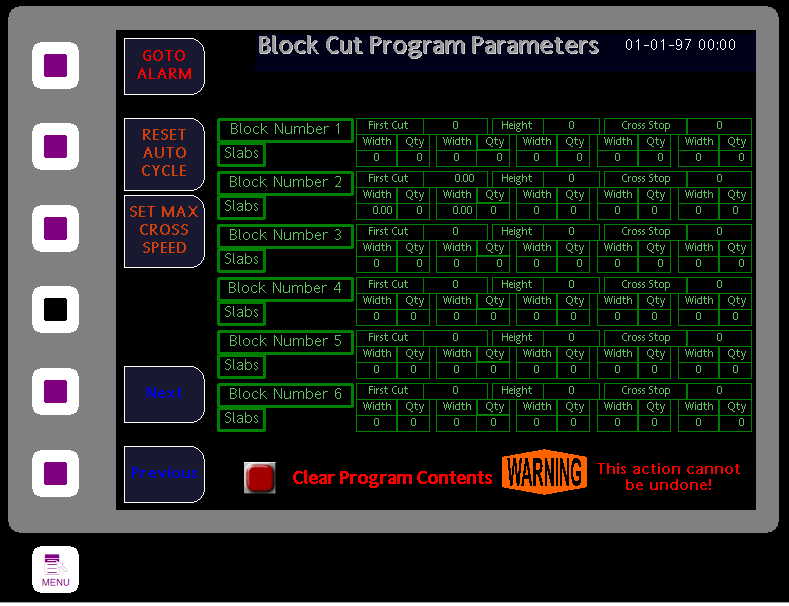
\includegraphics[width=0.5\linewidth]{screen-captures/program/pgm_review1}
	\caption{Programming - Check Program}
	\label{fig:prg-chk-prg}
\end{figure}
\section{Details}\paragraph*{The}\textbf{Check Program} screen details are divided into the following categories ...
\begin{list}{$\diamond$}{}
	\item \textbf{Screen Navigation}
	\item \textbf{Block Details}
	\item \textbf{Cycle Reset and Program Clear}
	\item \textbf{Set Max Cross Speed}
\end{list}
\pagebreak
\subsection{Screen Navigation}
\paragraph*{Is}performed by using the programmable Function Keys (FKeys) located down the left hand side of the OI Terminal (refer to Figure 9.2). Since this screen, and subsequent 	\textbf{\textit{CHECK PROGRAM}} screens are sub-screens of the \textbf{\textit{BLOCK PROGRAM}} screen, except for navigating to the \textbf{\textit{ALARM}} screen, navigation is from \textit{current screen} to \textit{next or previous screens}.The Operator may navigate to the following screens ...
\begin{list}{$\diamond$}{}
	\item \textbf{GOTO ALARM} Navigate to Alarm Screen.
	\item \textbf{SET MAX CROSS SPEED} Navigate to Cross Travel Global Speed Override screen.
	\item \textbf{NEXT} Navigate to next Check Program Screen.
	\item \textbf{PREV} Navigate to Block Program Screen, or if on Check Program Screen num 2 or higher, return to previous Check Program Screen.
\end{list}
\begin{figure}
	\centering
	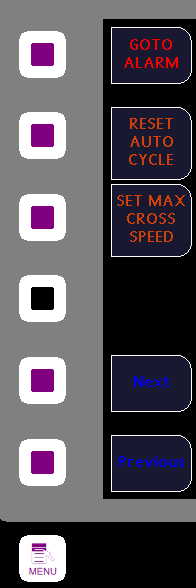
\includegraphics[width=0.2\linewidth]{screen-captures/program/pgm-review1-nav}
	\caption{Block Program Screen Navigation}
	\label{fig:pgm-reveiw1-nav}
\end{figure}
\paragraph{\textbf{\LARGE \textcolor{blue}{i}}}
The Menu Key located on the terminal at the lower left below the FKey's, will return the Operator to the Main Screen, from all other screens.\\
\begin{minipage}{4cm}
	\begin{picture}(20,70)
		
\includegraphics[width=.5\linewidth]{screen-captures/menu}
	\end{picture}
\end{minipage}\begin{minipage}[]{11cm}
	\paragraph{\textbf{\LARGE \textcolor{blue}{i}}} The Menu Key is pictured as it looks on the Terminal.
\end{minipage}
\pagebreak
\subsection{Block Details}\paragraph*{Blocks}as programmed,are shown in a table form (Figure 9.3).If a block has been programmed (based on the \textbf{\textit{Number of Blocks}}) it will be displayed, even if the details haven't been fully entered in the Block Program screen yet. The same applies to the slabs associated with that block. There is the ability to view up to six (6) blocks per \textbf{\textit{CHECK PROGRAM}} screen, and up to 5 different slab sizes per block. This allows viewing of up to 24 Blocks and up to 120 Slabs. In practical terms, it will likely never be used fully. The tabular form of the display of the block details, is similar in design to the paper forms currently used for machine setup details by the Operator. This should help when the Operator is reviewing the program details they entered for correctness, prior to running an automatic cycle using the programmed block data.
\paragraph{}
\begin{figure}
	\centering
	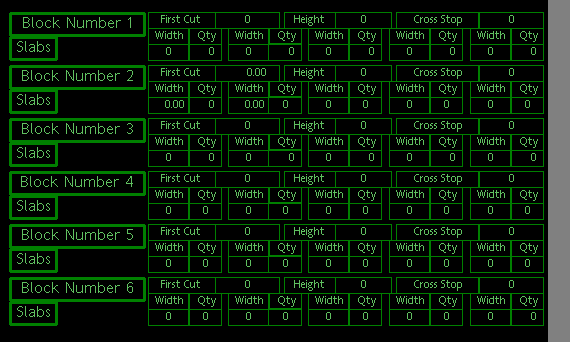
\includegraphics[width=.5\linewidth]{screen-captures/program/pgm_review1-block-data}
	\caption{Block Details Check Program}
	\label{fig:pgm-review-block-data}
\end{figure}
\paragraph{\textbf{\LARGE \textcolor{blue}{i}}}The Check Program pages are a useful tool to review the \textit{Block Program} that was entered in a table form which shows details about each block and slab. Also, it is \textbf{strongly advised} to \textbf{reset} \textbf{both} the \textit{block program} \textbf{and} \textit{the automatic sequence} \textbf{before} entering a new block program. This can be done on this \textbf{\textit{CHECK PROGRAM}} screen.
\paragraph{\textbf{{\LARGE \textcolor{red}{!}}}}A fault will be triggered by the program logic if the Operator tries to begin an Automatic Cycle without first entering a valid cut program. The Block Height is a critical dimension, if not correct, it can result in damage to the saw blade.
\subsection{Cycle Reset and Program Clear}\paragraph*{RESET AUTO CYCLE}PB is for the Operator to be able to reset the Automatic Sequence of Saw operation. This reset's control bit's that are used in tracking block completion, slab completion, and other intermediate operational data. This action should be performed even before entering a new block cutting program. By performing this operation, the Operator is ensuring the Saw is ready for a new program sequence to be run correctly.
\begin{figure}
	\centering
	
\includegraphics[width=.2\linewidth]{screen-captures/program/pgm_review1-aut-rst}
	\caption{Check Program - Auto Cycle Reset Button}
	\label{fig:pgm-review1-aut-rst}
\end{figure}
\paragraph{PROGRAM CLEAR}is for the Operator to clear out the Block Program Block and Slab data areas in the PLC (Controller). This wipes all data related to the Block Cutting Program that was currently in the Controller, reverting values to zero.
\begin{figure}
	\centering
	
\includegraphics[width=.3\linewidth]{screen-captures/program/pgm_review1-clr-pgm}
	\caption{Check Program - Clear Program Contents Button}
	\label{fig:pgm-clr}
\end{figure}
\paragraph{\textbf{\LARGE \textcolor{blue}{i}}}The Operator will be prompted by an \textit{accept or cancel popup}, to either \textsl{accept clearing the program}, or \textsl{resetting the sequence}, or \textsl{cancel the operation}. This is an \textbf{immediate action} and \textbf{cannot be undone}.
\subsection{Set Max Cross Speed}\paragraph*{Cross Travel Speed Override}capability is intended to be used when the Operator desires to limit the cutting speed of the saw during automatic operation. It's primary function is to provide the ability to \emph{run in} the newly installed segments of the saw blade. When selecting this navigation key it will open the \textbf{\textit{Set Maximum Cross Travel Speed}} screen (Fig. 9.6).

\paragraph{\textbf{\LARGE \textcolor{blue}{i}}}The Operator will be able to Enable/Disable the Cross Travel Speed Override and set the Maximum Cross Travel Speed from the \textbf{\textit{Set Maximum Cross Travel Speed}} screen when they select this Navigation Key.

\subsection{Set Maximum Cross Travel Speed Screen}\paragraph*{Enable/Disable Speed Override}referring to Figure 9.6 Speed Override is achieved by pressing the toggle button provided on the screen. The toggle has a corresponding state indicator to show whether it is enabled or disabled at the present time. The Operator can also set the speed limit of the override which is represented in feet per minute. Simply pressing the number displayed will open a setting keypad onscreen to use for entry.
\begin{figure}
	\centering
	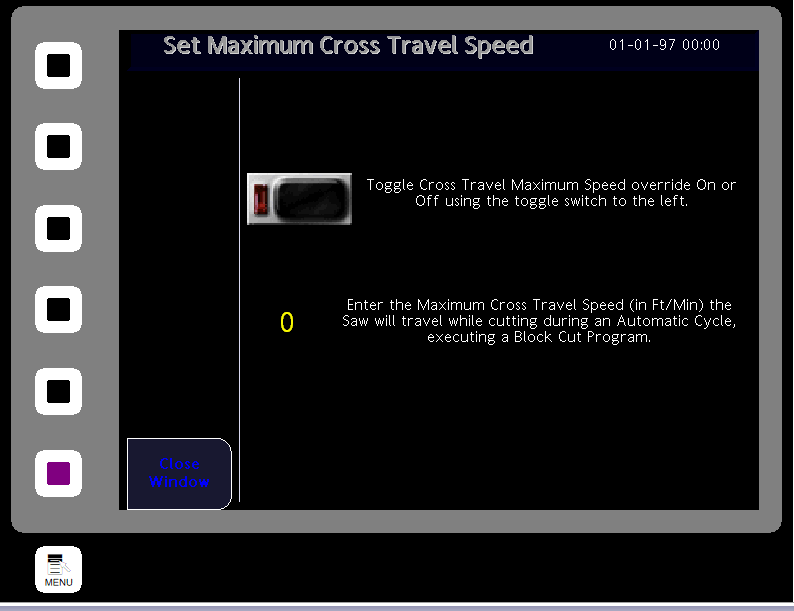
\includegraphics[width=.8\linewidth]{screen-captures/program/global_speed}
	\caption{Cross Travel Speed Override Screen}
	\label{fig:global_speed}
\end{figure}
\paragraph{\textbf{\LARGE \textcolor{blue}{i}}}The Operator will be able to use this setting to limit maximum speed of the Cross Travel motion during cutting operations. This is an \textit{Immediate Acting} setting which directly affects the speed which the saw blade moves through the stone. The indicator takes time to update it's state on the display screen, even though it has changed state, this is a result of the communication between the PLC and HMI